\problemname{Bike Parking}

Sanne recently conceived a lucrative business idea: renting out premium bike parking at the Eindhoven train station.
To maximize her profits, she divided the bike parking slots into $N$ different tiers, numbered from $0$ to $N-1$.
Tier 0, the premium tier, is located very close to the train platforms.
Higher-numbered tiers consist of parking slots that are worse (the higher the tier, the worse the slot).
The number of slots in tier $t$ is $x_t$.

Users parking their bikes are assigned their parking slot via an app.
Each user has a subscription level and expects a parking slot in the corresponding tier.
However, the terms of service do not guarantee users a slot in their respective tier.

If a user with subscription level $s$ is assigned a slot in tier $t$, then one of the following three things happens:
\begin{enumerate}
\item If $t < s$, the user will be happy and upvote the app.
\item If $t = s$, the user will be satisfied and will not do anything.
\item If $t > s$, the user will be angry and downvote the app.
\end{enumerate}

Today, Sanne's app has $y_0+y_1+\ldots+y_{N-1}$ users, where $y_s$ is the number of users with subscription level $s$.
She needs your help to assign the users to the parking slots. Each user should get exactly one
slot. No slot can be assigned to more than one user, but it is okay for some parking slots to not be assigned to any users. Furthermore, the total number of users does not exceed the total number of available parking slots.

Sanne wants to maximize the rating of her app.
Let $U$ be the number of upvotes and $D$ be the number of downvotes.
Your task is to maximize $U-D$.

\section*{Input}
The first line contains one integer $N$, the number of tiers or subscription levels.

The second line contains $N$ integers $x_0, x_1, \ldots, x_{N-1}$,
the number of slots in the different tiers.

The third line contains $N$ integers $y_0, y_1, \ldots, y_{N-1}$,
the number of users with each subscription level.

\section*{Output}
Output one integer, the maximum possible value of $U-D$ by assigning the users to parking slots optimally.

\section*{Constraints and Scoring}
\begin{itemize}
\item $1 \leq N \leq 3 \cdot 10^5$.
\item $0 \leq x_i, y_i \leq 10^9$ for $i = 0,1,\ldots , N-1$.
\item $y_0+y_1+\ldots + y_{N-1} \leq x_0+x_1+\ldots + x_{N-1} \leq 10^9$.
\end{itemize}

Your solution will be tested on a set of test groups, each worth a number of points.
Each test group contains a set of test cases. To get the points for a test group, you need to
solve all test cases in the test group.

\begin{tabular}{|l|l|l|}
\hline
Group  &  Score  &  Limits \\
\hline
 1 & 16 & $N=2, x_i \leq 100, y_i \leq 100$ \\
\hline
 2 & 9 & $x_i = x_j = y_i = y_j$ for all $i,j$. In other words all the $x$'s and $y$'s in the input are the same. \\
\hline
 3 & 19 & $x_i, y_i \leq 1$ \\
\hline
 4 & 24 & $N,x_i,y_i \leq 100$  \\
\hline
 5 & 32 & No additional constraints. \\
\hline
\end{tabular}
\section*{Examples}
Note that some of the samples are not valid input for all test groups.
The $i$th sample is at least valid for the $i$th test group.

In the first sample, you can assign the user with subscription level 0 to a tier 0 slot,
assign two users of level 1 to tier 0 slots (leading to 2 upvotes), and assign the
remaining level 1 user to a tier 1 slot. This leads to a rating of $2$.

In the second sample, you can assign the level 1 user to the tier 0 slot, the level 2 user
to the tier 1 slot, and the level 0 user to the tier 2 slot. This gives 2 upvotes and
1 downvote, leading to a rating of $1$.

In the third sample, you can assign the level 1 user to the tier 0 slot, the level 0 user
to the tier 2 slot, and the level 4 user to the tier 3 slot. This again gives 2 upvotes and
1 downvote, leading to a rating of $1$.

The fourth sample is illustrated below. You can assign the users of level 1 to slots of tiers 0, 0, 3 and 3, leading
to 2 upvotes and 2 downvotes. Next, assign the users of level 2 to slots of tiers 1, 2, 3 and 3,
leading to 1 upvote and 2 downvotes. This amounts to 3 upvotes and 4 downvotes, so the rating is $-1$.

\begin{figure}
\centering
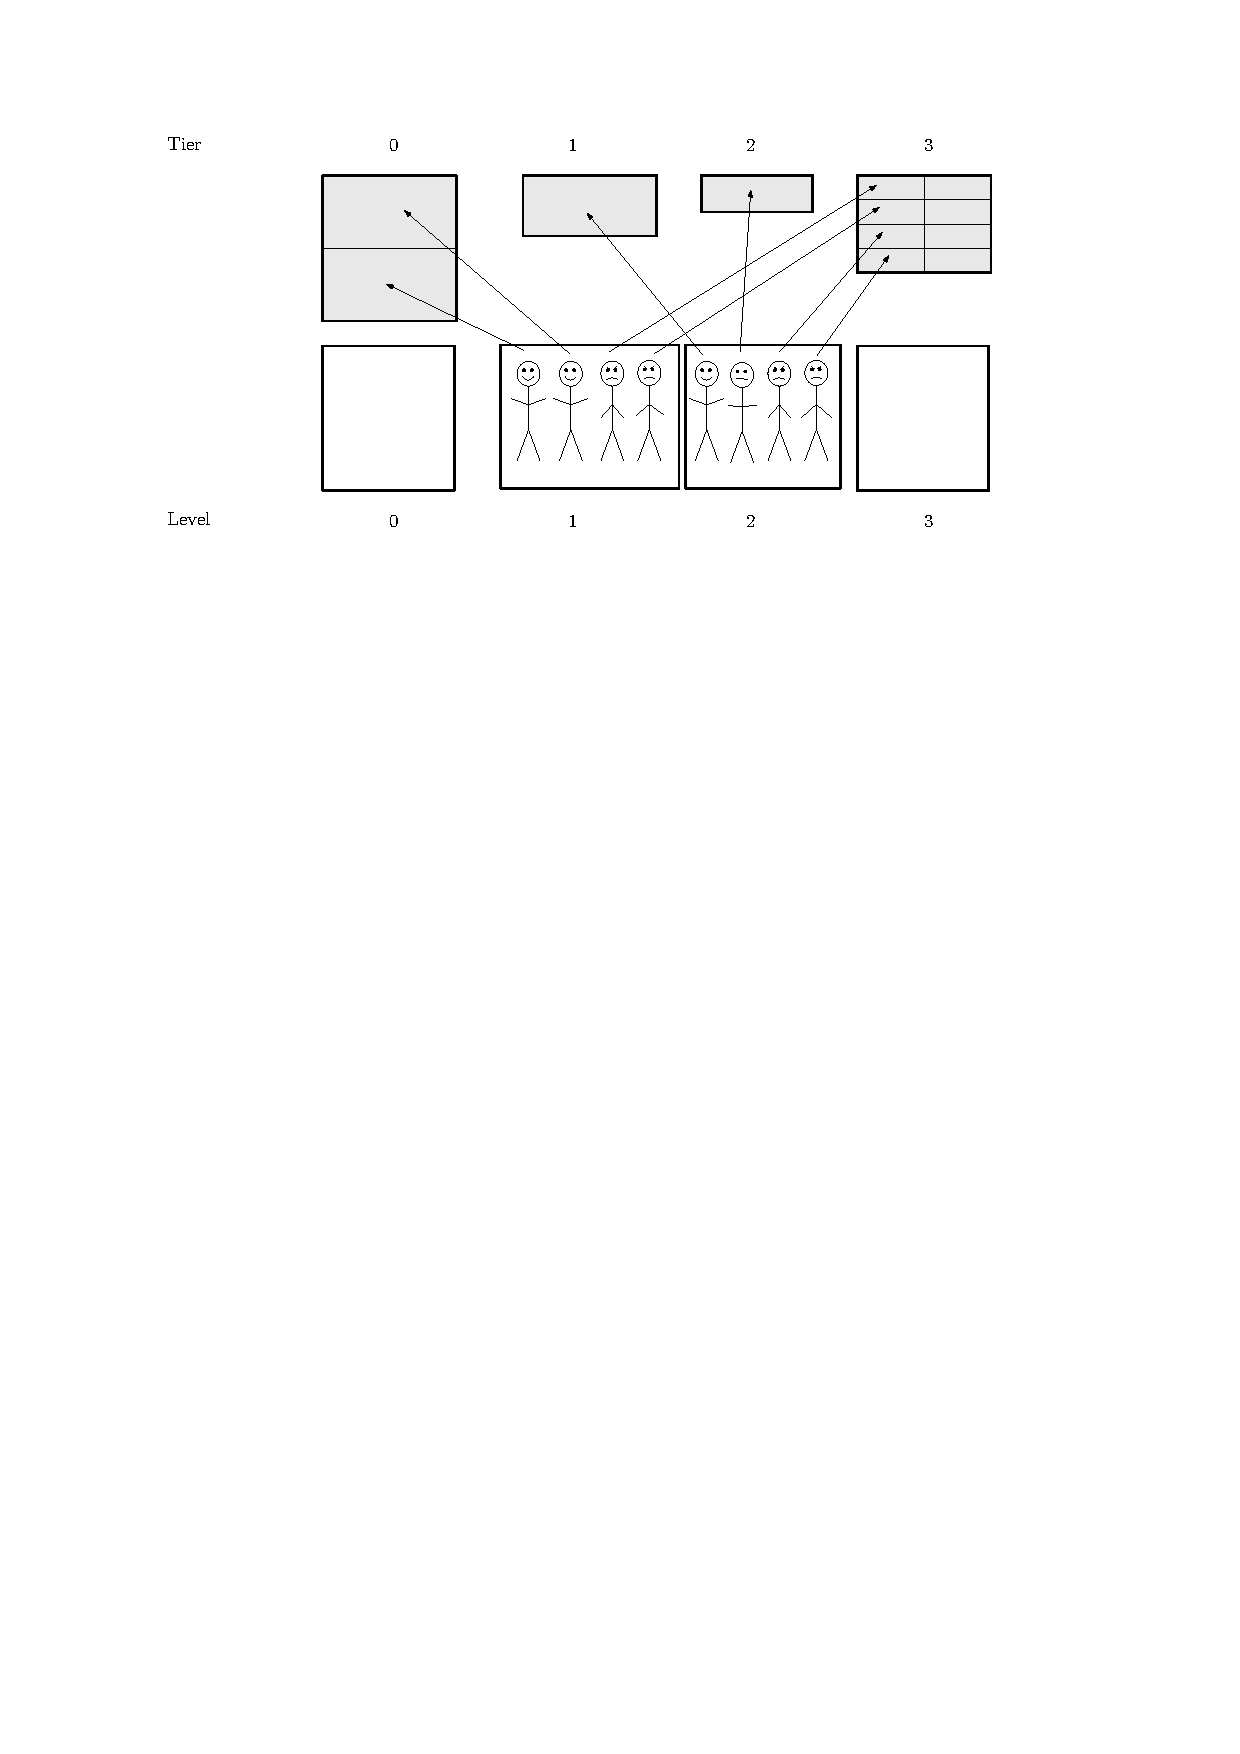
\includegraphics[width=0.7\textwidth]{sample.pdf}
\end{figure}

In the fifth sample, you can assign everyone to a slot matching their own subscription level,
so the rating is $0$.
